\section{Introduction}

\Acp{AED} are normally used to treat epilepsy.
One third of epilepsies are drug-resistant \cite{engel_what_2016}.
Curative resective surgery can be performed to remove the \ac{EZ} (\cref{chap:resection}).
The location of the \ac{EZ}, ``the area of cortex indispensable for the generation of clinical seizures'' \cite{rosenow_presurgical_2001}, is normally inferred by a multidisciplanary team following non-invasive evaluation such as video-\ac{EEG}, \ac{MRI} or neuropsychological tests.
If the information regarding the location of the \ac{EZ} is discordant between the different tests, \ac{iEEG} electrodes may be implanted to localize it precisely.
To determine the brain regions that need to be recorded, i.e., the targets for the \ac{iEEG} electrodes, the team leverages information from the non-invasive examinations, including seizure semiology from the recorded videos (\cref{chap:videos}).
The choice of targets is therefore influenced by the team's subjective experience and personal knowledge of the literature.
This leads to substantial variations of implantation strategies across different epilepsy centers \cite{tufenkjian_seizure_2012}.
The diagnostic pathway for surgical planning could be supported by an objective tool to aid clinicians in deducing the \ac{EZ} location from seizure semiology.

% One way to plan the implantation objectively is developing a data-driven, automated method.
% We performed a systematic literature review to generate an open-access database containing ``11230 datapoints from 4643 patients across 309 articles'', where each datapoint represents a patient showing a certain semiology who became seizure-free after resection of a certain brain structure \cite{alim-marvasti_probabilistic_2021} (\cref{fig:semiology_review}).
% In this context, seizure-free refers to one full year without seizures after resective surgery.
% The database, called \svtdatabase, can be queried to quantitatively map observed seizure semiologies to brain structures that were removed leading to seizure freedom.
% The brain structures included in \svtdatabase are extracted from the Neuromorphometrics atlas%
% \fnurl{http://www.neuromorphometrics.com}.
% \Cref{tab:single_semiology} shows a conceptual usage example.

% \begin{figure}
%   \centering
%   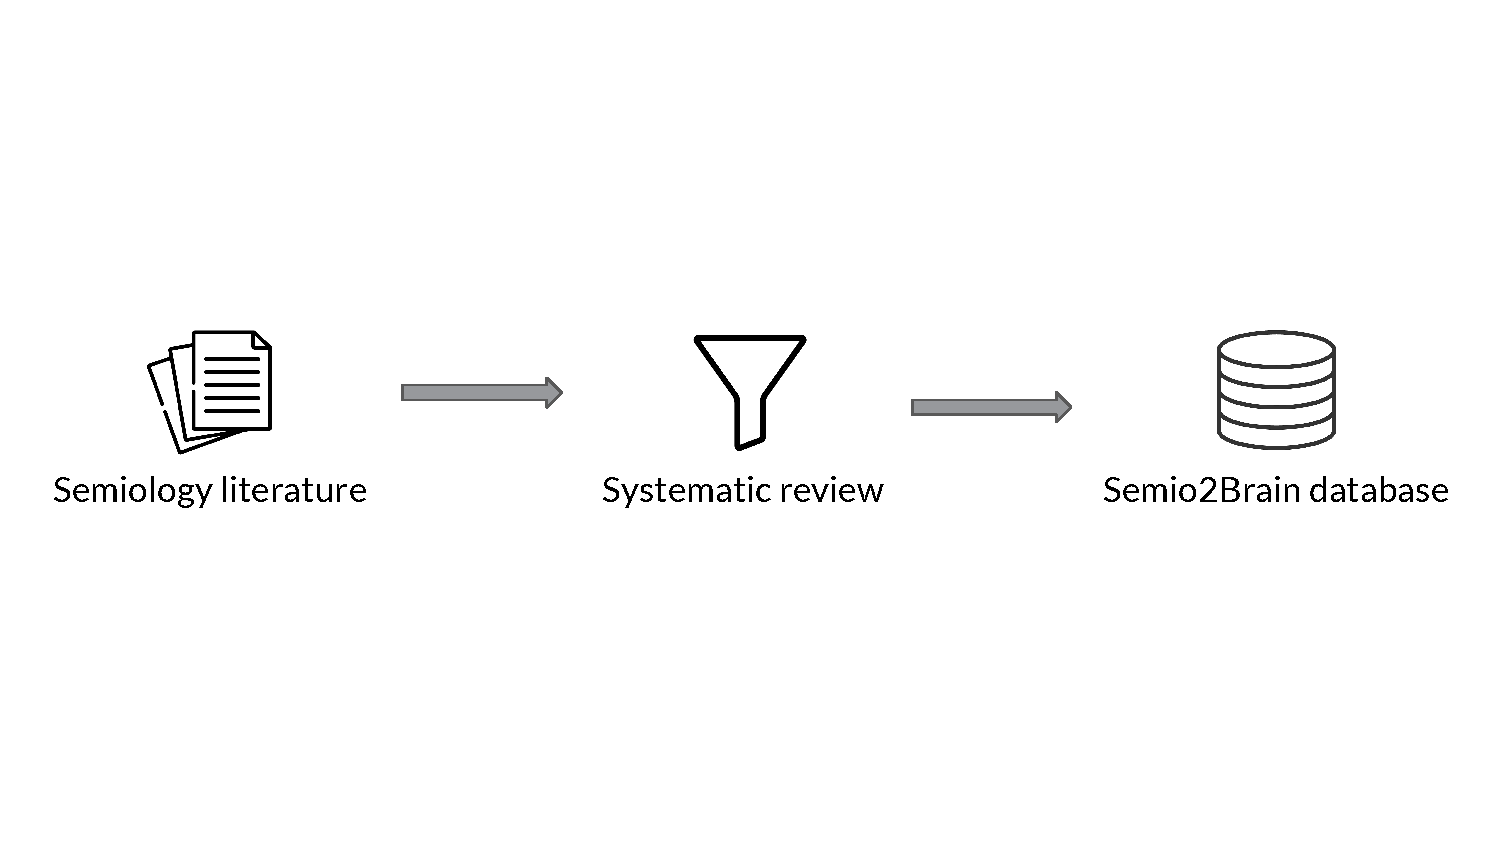
\includegraphics[trim=0 150 0 150, clip, width=\linewidth]{svt_1}
%   \caption[Systematic semiology literature review to build the \svtdatabase database]{
%     Systematic semiology literature review to build the \svtdatabase database.
%   }\label{fig:semiology_review}
% \end{figure}

Researchers who do not wish to code would benefit from a \ac{GUI} to query the database.
Moreover, visualizing the probability of each structure containing the \ac{EZ} on \ac{3DMMI} could help plan the resection and \ac{iEEG} implantation strategies \cite{nowell_resection_2017, nowell_utility_2015}, potentially using \ac{ATP} \cite{sparks_automated_2017}.
Finally, a \ac{3DMMI} visualization could be used to perform qualitative and quantitative analyses of the retrospective information contained in the \svtdatabase.

In this work, we present a software tool that, given an observed list of seizure semiologies and other patient data such as the dominant hemisphere, generates a table with the number of datapoints associated to each brain region.
Each datapoint represents a patient presenting the observed semiologies who became seizure-free after resection of the corresponding brain structure (\cref{tab:single_semiology}).
The usage examples in this thesis use the \svtdatabase database and the corresponding software used to query the database \cite{alim-marvasti_probabilistic_2021,alim-marvasti_mapping_2021}, which were defined based on the Neuromorphometrics atlas parcellation%
\fnurl{http://www.neuromorphometrics.com}.

\begin{table}
  \setlength{\tabcolsep}{3pt}
  \centering
  \caption[Result of querying an imaginary database with one semiology]{
    Result of querying an imaginary database with the semiology \textit{Head version} and exemplar brain structures A, B and C, assuming that the brain has been parcellated into only three structures.
    In this example, according to the literature analyzed to build the database, structure C was one of the resected structures in 20 patients presenting \textit{Head version} who became seizure-free after surgery, suggesting a high probability of the \ac{EZ} being associated with that structure.
    Structure B was resected for five patients who became seizure-free after surgery.
    Structure A was never resected in patients who presented \textit{Head version} and became seizure-free after surgery.
    This result would support the decision of implanting electrodes in structure C (and possibly B), as they are likely to be associated with the \ac{EZ} according to the retrospective information in the literature.
    The actual list of brain structures would depend on the method used to parcellate the brain.
  }
  \label{tab:single_semiology}
  \begin{tabular}{l*3c}
    \toprule
                          & \textbf{Structure A} & \textbf{Structure B} & \textbf{Structure C} \\
    \midrule
    \textbf{Head version} &                    0 &                    5 &                   20 \\
  \end{tabular}
\end{table}

% In this work, we present our software tool to visualize the \ac{EZ} probability map on \ac{3DMMI}.
% Show example of multiple semiologies and aggregation
% Details on the methods used for aggregation are out of the scope of this thesis
